\chapter{André Martinet and Functional Phonology}
\label{ch.martinet}

If we take the views of the {Prague School} linguists
(chapter~\ref{ch.prague}) to represent the core of European
Structuralism between the two world wars, it is apparent that
Glossematics (chapter~\ref{ch.hjelmslev}) constitutes a significant
departure.  While the work of \name{André}{Martinet} to be considered below is
generally seen as a natural continuation of Praguian phonology, his
views are also distinct in some ways. {\Martinet} was certainly close to
the {Prague School}, but he was also a friend of Louis {\Hjelmslev}, and
their interaction also influenced him.  In their relationship, there
is an interesting symmetry in that one of the languages whose sound
structure {\Hjelmslev} treated was that of {\Martinet}, \ili{French}, while one of
those that formed part of the basis for {\Martinet}'s Doctorate was
{\Hjelmslev}'s \ili{Danish}. {\Martinet}'s relationship with {\Jakobson} was
especially complex: they were close for some years, but later fell
out, and much of {\Martinet}'s intellectual agenda developed as
repudiation of {\Jakobson}ian positions.


\section{Martinet's life and career}
\label{sec:martinet-life}

\name{André}{Martinet} was born in Saint-Alban-des-Villards, in Savoy (France)
on 12 April 1908.\footnote{\posscitet{martinet93:memoires}
  \textsl{Mémoires} provide a great deal of information about his life
  and career which I have made use of in the present section. Where
  facts from his life are cited without attribution, this is generally
  the source from which I have derived them.} His parents were
schoolteachers, and he spent his childhood in an environment where the
local language was a \ili{Franco-Provençal} patois: he describes his
mother's language in \citealt{martinet56:description} as an application
of his theory of phonological description.  The language of education,
however, both among the educated and in addressing those not
considered ``locals'' (including {\Martinet}, whose family was originally
from a village not among those in which they lived) was the local form
of standard \ili{French}. He was thus sensitized to the nature of bilingual
communities, and thereby to matters of language, from an early age.

When he was eleven, his family moved to Paris, where he continued his
education through lycée and university. At the Sorbonne from 1925 to
1930 he studied \ili{English} and \ili{Germanic}, including a course in Old Norse
with \name{Paul}{Verrier} (1860--1938) which he particularly enjoyed. {\Verrier}
recommended him for a fellowship to attend a summer course in {Danish}
in Copenhagen in the summer of 1928, and this began {\Martinet}'s long
connection with Denmark and {Danish} linguists.

\begin{wrapfigure}{r}{.35\textwidth}
  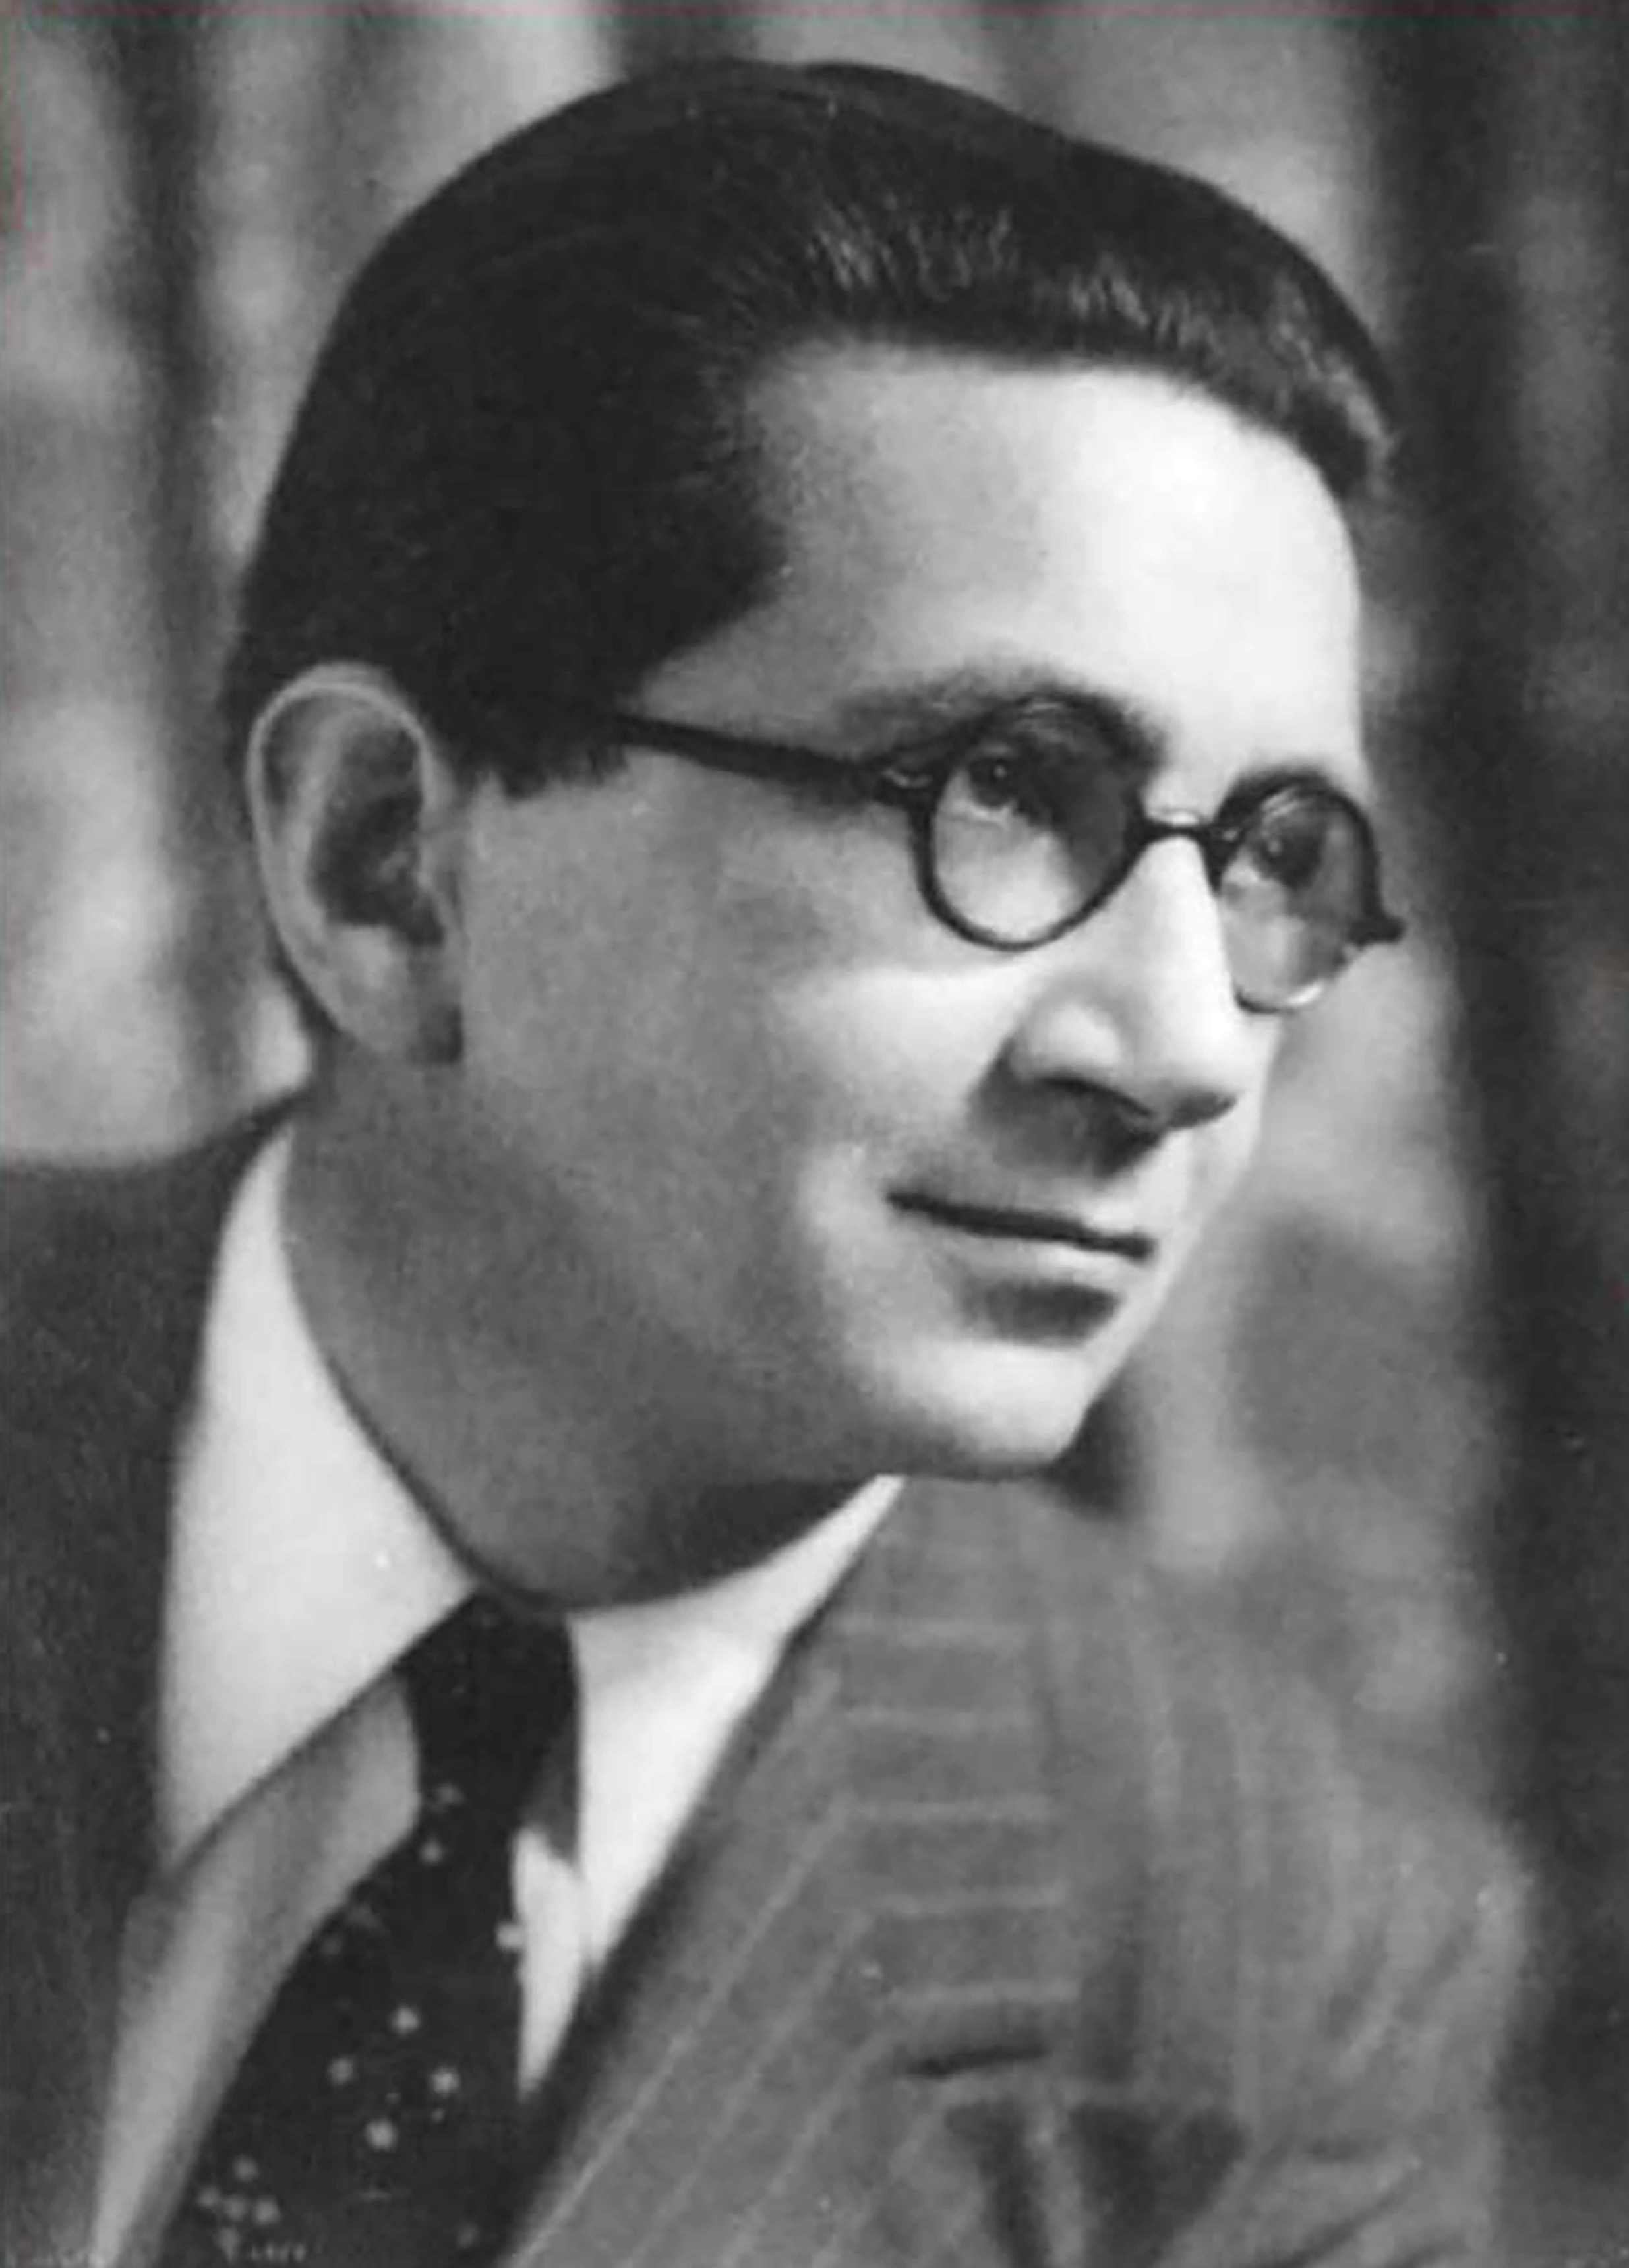
\includegraphics[width=.9\textwidth]{figures/martinet-0.jpg}
  \caption{André Martinet}
  \label{fig:ch.martinet.martinet0}
\end{wrapfigure}
In 1930, he passed the requirements for the `agrégation' in {English}, a
selective and highly competitive examination which authorizes those
accepted to teach at higher \isi{levels} in lycées and universities.  After
teaching briefly at the lycée in Poitiers, he spent most of 1932--34
in Berlin, where he began work on the first of two required
dissertations for the Doctorate \citep[][on \ili{Germanic} consonant
gemination]{martinet37:thesis}.  On one of his numerous visits to
Denmark, in the summer of 1933 he met \name{Karen}{Mikkelsen-Sørensen}, whom
he would marry the following year, one of the witnesses at their civil
ceremony being \name{Otto}{Jespersen}: ``In Copenhagen in 1934, {\Martinet} met
\name{Otto}{Jespersen}, whom he admired both as an outstanding linguist and
anglicist and as an interlinguist and creator of the planned language
project Novial'' \citep[276]{klare12:martinet}.  He had translated
\posscitet{jespersen22:language} book \textsl{Language} into
{French}---though while \citet[158]{martinet91:bio} says that the
translation had ``retardé d'un an [son] succès à l'agrégation'', there
is no evidence that these efforts ever led to this translation being
published.

Around this time, he became interested in the work of the Prague
School linguists, and read the first several numbers of their
\textsl{Travaux} with interest. At the 1935 London Congress he met
{\Trubetzkoy}, with whom he subsequently corresponded. In his summary
letter to {\Jakobson} after that meeting
\citep[246--248]{liberman01:trubetzkoy.anthology}, {\Trubetzkoy} is very
positive about {\Martinet}, who he says ``is quite ``ours'', despite
{\Hjelmslev}'s efforts to ``convert'' him.''
\posscitet{martinet36:neutralization} article ``Neutralisation et
archi\-pho\-nème'', was published in the volume 6 of the Prague
\textsl{Travaux}.  His frequent stays in Denmark also resulted in
connections with {Danish} linguists including Louis {\Hjelmslev} and Hans
{\Uldall}, and he discussed with them the evolving theory of Glossematics
(chapter~\ref{ch.hjelmslev}). His \citeyear{martinet46:rvw.hjelmslev}
review of \citealt{hjelmslev43:prolegomena} in the \textsl{Bulletin de
  la Société de linguistique de Paris} contributed significantly to
making {\Hjelmslev}'s views known outside of Denmark.

His second, ``complementary'' thesis \citep{martinet37:danish} on the
phonology of \ili{Danish}, completed on the basis of work with his wife
Karen\ia{Mikkelsen-Sørensen, Karen}, is one of the first substantial 
descriptions of a language on
the basis of Praguian views. On the basis of these two works, he
obtained his doctoral degree, and was then appointed in the autumn of
1937 to a teaching post as director of phonological studies at the
École pratique des Hautes Études at the Sorbonne.

On the outbreak of the war in 1939, {\Martinet} was recalled to military
service, where he was designated as an interpreter of \ili{Danish} (the only
one in the \ili{French} army). After some delay, his unit was sent to the
Somme front in June of 1940, where they were promptly encircled and
captured by the Germans, and sent off to prison camp at
Weinsberg. Although not holding an appropriate rank, his status as a
translator (controlling \ili{French}, \ili{German} and \ili{English}) was ambiguous
enough for him to be interned in a camp for officers, allowing him to
stay together with a group of officers from a wide variety of regions
in France. During his time in the Weinsberg camp, he took advantage of
this situation to collect data on \isi{phonological variation} in spoken
\ili{French} which he published as \citealt{martinet45:french}.

{\Martinet} spent only a year and three months in the prison camp. His
wife\ia{Mikkelsen-Sørensen, Karen} had taken a job in a {German} bookstore 
in occupied Paris, and
petitioned the occupation authorities for his release, which was
granted. He returned to Paris in October, 1941, and resumed his
teaching at the École pratique des Hautes Études. The circumstances of
his release, however, cast a shadow of potential collaboration with
the Germans, for which he was denounced when France was liberated;
this led to a request that he stop teaching at the Sorbonne, though he
continued his classes in private. The charge of collaboration was
eventually withdrawn, partly on the basis of support he had provided
for a friend in the resistance who was hiding from the Gestapo.

He was not, however, freed of all suspicions, and his position among
his colleagues in Paris was somewhat difficult. Although he took up
his teaching once more in October of 1945, this history no doubt
played a role in his not being appointed, on the retirement of Joseph
{\Vendryes}, to the one chair in linguistics that existed in the
Sorbonne, with the appointment instead going to a less well known
Indo-Europeanist, \name{Michel}{Lejeune}
\citep{joseph16:martinet.weinreich}. Partially in reaction to this
slight, it seems, when he was offered in 1946 a position directing
research at the International Auxiliary Language Association in New
York, he accepted and left Paris for the US the following year.

At the end of the war, {\Martinet} and his wife 
Karen\ia{Mikkelsen-Sørensen, Karen} had found it
difficult to re-establish their domestic life, and they
separated. Karen\ia{Mikkelsen-Sørensen, Karen} returned to Denmark 
with her daughter Hanne by her
first marriage, and {\Martinet} and their daughter Catherine remained in
Paris.  There he met \name{Jeanne}{Allard}, a student in his phonetics class
and a researcher in her own right. They eventually came to live
together, and were married in New York in April, 1947, a month after
his divorce from Karen became final.

The war had seen the effective dissolution of the Prague
School. {\Trubetzkoy} had died in 1938; {\Jakobson} had fled to New York,
and those linguists who remained in Czechoslovakia were difficult to
contact.  {\Martinet}'s own maintenance of a notion of phonology derived
from Praguian ideas thus took on a more distinctive role.

In New York, he was in contact with {\Jakobson}, whom he had first met at
the 3rd International Congress of Phonetic Sciences in Ghent in 1938.
{\Jakobson}, as a part of his efforts to counter the isolationism of
American linguistics by promoting European scholars, exerted his
influence at Columbia to obtain the then-vacant chair of general and
comparative linguistics there for {\Martinet} in 1947, effectively making
him head of the (quite small) department as of 1948, once he had
finished his obligations to the IALA.  At Columbia, he taught not only
general synchronic linguistics but also comparative and {Indo-European}
linguistics. His theory of the nature and motivation of linguistic
change, to be addressed in section~\ref{sec:economie} below, was
developed in
\citealt{martinet52:function.structure,martinet55:economie}.

During this period he also became editor of \textsl{Word}, the journal
of the \isi{Linguistic Circle of New York}, one of whose founders in 1943
was {\Jakobson}. Initially responsible for articles submitted in {French},
together with \name{Morris}{Swadesh} (whose qualities as a linguist he
appreciated much more than as an editor) who dealt with those in
{English}, he continued after {\Swadesh}'s departure to direct the journal
in collaboration with \name{Joseph}{Greenberg}, \name{Uriel}{Weinreich} and finally
\name{Louis}{Heller} until 1965, even after he left New York.

By 1954, {\Martinet}'s relations with administrators and others at
Columbia had become rather tense. In part this resulted from his
efforts to secure support for the creation of a chair in Yiddish
Studies, to be occupied by his student \name{Uriel}{Weinreich}, and in part
from conflicts with \name{John}{Lotz}, a {Hungarian} scholar and member of the
Columbia faculty whom the administration wished to have join
{\Martinet}'s Department of Linguistics. These matters so disturbed
{\Martinet} that he determined to leave New York and return to France.

As \citet{joseph94:rvw.martinet} notes, there is some irony in the
fact that part of the problem he had at Columbia resulted from his
efforts to promote a chair in Yiddish Studies, a goal of which his
Jewish colleagues would presumably have been supportive.  As observed
by Joseph\ia{Joseph, John} \citep[and also by][]{auroux93:martinet,goldsmith98:rvw.barsky},
a number of passages in \posscitet{martinet93:memoires}
\textsl{Mémoires} evidence a casual stereotyping and caricature that
imply an anti-semitism which is hard to accept and somewhat at odds
with his attitude toward {\Weinreich} (though see
\citealt{joseph16:martinet.weinreich} for some discussion of their
relationship). This is particularly manifest in connection with his
early strong animus toward {\Chomsky}.

\citet[30f.]{martinet94:word} recounts with glee the fact that in
1957, he over-ruled his co-editor {\Weinreich} to reject a paper of
{\Chomsky}'s---according to \citet[347]{murray99:gatekeepers}, the only
time {\Chomsky} ever had a journal submission rejected. {\Martinet} says
that the rejected paper was ``a first version of \textsl{Syntactic
  Structures}'', a characterization which is quite implausible given
the facts that (a) \citealt{chomsky57:ss}, at 118 pages, is hardly
something that would have been submitted for journal publication in
the 1950s; and (b) the book had already been published by Mouton early
in 1957.  \citet[132]{chomsky79:lg.and.resp} recalls that the paper in
question was ``a technical article on \isi{simplicity} and \isi{explanation}''
which {\Jakobson} had suggested he send to \textsl{Word}; Apparently the
paper ``[was] ``Simplicity and the Form of Grammars'', written in the
mid-1950s, which spelled out the logic Noam\ia{Chomsky, Noam} discussed at length in
\textsl{Morphophonemics of Modern Hebrew}
{[\citealt{chomsky51:mmh}]}. Alas, ``Simplicity and the Form of
Grammars'' has been lost to history.'' (p.c., \name{Jeffrey}{Watamull} 
to \name{Bert}{Vaux}, 25 July, 2021)

{\Martinet}'s imperfect memory when it came to scholars with whom he was
unsympathetic was also displayed with regard to \name{Morris}{Halle}. In a
discussion about how well he might actually have known {\Chomsky}, he
observes that ``[i]l ne me pardonnait pas la réjection de l'article
qu'il avait envoyé à \textsl{Word}. Celui que je connaissais bien, en
revanche, c'était son collaborateur \name{Morris}{Halle}; le seul de mes
étudiants américains que j'aie jamais collé''
\citep[69]{martinet93:memoires}.\footnote{``he [{\Chomsky}] did not
  pardon me for the rejection of the article he had sent to
  \textsl{Word}. The one I knew well, however, was his collaborator
  \name{Morris}{Halle}, the only one of my American students that I ever
  failed.''} There is no evidence that {\Chomsky} was particularly upset
about the rejection of his article, but on the other point, {\Martinet}
was apparently fond of recounting how he had failed {\Halle} at
Columbia. And {\Halle} was apparently fond in his turn of retelling this,
and confronting it with the transcript of his actual academic record
for that term at Columbia, where he received a grade of ``A'' from
{\Martinet}.\footnote{I am indebted to \name{Bert}{Vaux} for this anecdote.}

During the same period, {\Martinet}'s relations with {\Jakobson} had become
notably less warm. His own thinking about linguistic matters, and
phonology in particular, led him to reject {\Jakobson}'s program of
universal structures and binary \isi{oppositions} in favor of a much more
particularist approach to individual languages. Owing his position at
Columbia and his role at \textsl{Word} to {\Jakobson}, however, he was
not interested in provoking open conflict. Nonetheless, over the
ensuing years matters came to such a point that neither was willing to
participate in events where they were likely to share attention with
the other, and their direct contacts became limited to accidental
encounters.  {\Chomsky}'s speculation (p.c., 26 May, 2021) that the
rejection of his article mentioned above ``had to do with a feud
between [{\Martinet}] and {\Jakobson}'' is probably correct.

In 1955 {\Martinet} returned to France, though he was not able to resume
his original position at the École pratique des Hautes Études. A new
position as director of studies in structural linguistics was,
however, created for him there and he was able to re-establish himself
in Paris. \name{Michel}{Lejeune} designated him as his successor to the chair
in General Linguistics at the Sorbonne, but although {\Lejeune} retired
from the chair in 1955, {\Martinet}'s actual accession to the
professorship was held back until 1960.\footnote{The chronology here
  is difficult to establish in detail. Although the CV in
  \citealt[365f.]{martinet93:memoires} characterizes him as
  ``Professeur de linguistique générale à la Sorbonne 1955--1977'',
  \citet[79]{martinet93:memoires} refers to his advancement being
  blocked until 1960. This is supported by the fact that the title
  page of \citealt{martinet56:description} identifies the author
  simply as ``Directeur d'études à l'École pratique des Hautes
  Études'', but that of \citealt{martinet60:elements} identifies him
  as ``Professeur à la Sorbonne''.}

His classes for undergraduates at the Sorbonne resulted in the
publication of \citealt{martinet60:elements}, a work whose title was
intended to evoke that of {\Saussure}'s \textsl{Cours}. This introduction
to {\Martinet}'s development of his Saussurean and Praguian views was
immediately quite popular, and it has since been translated into more
than a dozen languages.  In 1965, he founded the journal \textsl{La
  Linguistique}, devoted to functionalist work; he continued to edit
the journal up through his final illnesses in the late 1990s.

In the aftermath of the events in France of May, 1968 and the
re-organization of the University of Paris into 13 separate
universities, {\Martinet} and his immediate colleagues in linguistics
were associated with the new Paris V, René Descartes University
(merged in 2019 with Paris VII to form the current University of
Paris). {\Martinet} retired as Emeritus Professor in 1977, though he
continued to lecture at the École pratique des Hautes Études until
1995. He died on 16 July 1999 in Châtenay-Malabry, France.

Over a long career, {\Martinet} trained a large number of scholars, first
at Colum\-bia and then through his seminars at the École pratique des
Hautes Études and his classes at the Sorbonne and elsewhere. He was
widely recognized as the foremost representative of structuralist
linguistics in France, and received a number of honorary degrees and
other honors. His views on synchronic matters and the theoretical
basis of phonology are central to functionalist theories, and continue
to have their adherents (see
\citealt{akamatsu92:essentials,akamatsu09:martinet} for example)
within a somewhat limited circle. His work on the theory of diachronic
change, on the other hand, and especially
\citealt{martinet52:function.structure,martinet55:economie} which will
be discussed below in section~\ref{sec:economie}, has been more widely
influential.

%\newpage
\section{Phonology as functional phonetics}
\label{sec:functional-phonetics}

\citet[93]{martinet93:memoires} speaks of ``le principe de base de la
linguistique structurale post-saussurienne, selon lequel un élément
n'existe que de ce qui le distinque des autres éléments du même
système''\footnote{``the basic principle of post-Saussurean structural
  linguistics, according to which an element only exists by virtue of
  what distinguishes it from the other elements of the same system''
  (my translation --- SRA)}, and much the same principle can be
invoked with respect to linguistic theories: their existence takes on
importance in relation to their distinctness from other theories of
the same domain. {\Hjelmslev}'s Glossematics differed from the Prague
School program of {\Trubetzkoy} and {\Jakobson} in rejecting a phonetic
basis for phonological \isi{oppositions}. {\Jakobson}, in turn, took issue with
{\Hjelmslev}'s extreme degree of abstraction in characterizing
phonological systems. For his part, {\Martinet} objected both to
{\Hjelmslev}'s \isi{abstractness} and to {\Jakobson}'s universalism and his
embrace of the principle of binary \isi{oppositions}. {\Martinet} also notes
his rejection as editor of \textsl{Word,} as noted above, of an early
submission by Chomsky, and stresses that he never had any sympathy
whatever for Chomsky's views. {\Martinet}'s own stance, then, is perhaps
a particularly clear example of a theory whose significance is based
on what separates it from others.

{\Martinet}'s views on phonology derive from his general picture of the
nature of human language, as presented for example in his
\textsl{Elements of General Linguistics}:\footnote{Citations of this
work are given from the readily available {English} translation rather
than from the {French} original.}
\begin{quotation}
  A language is an instrument of communication in virtue of which
  human experience is analysed differently in each given community
  into units, the monemes, each endowed with a semantic content and a
  phonic expression. The phonic expression is articulated in its turn
  into distinctive and successive units. These are the phonemes, of
  limited number in each language, their nature and mutual relations
  varying from one language to another.

  This implies (1) that we must reserve the term language to describe
  an instrument of communication with this twofold \isi{articulation} and
  vocal manifestation; (2) that outside this common basis there is
  nothing linguistic in the proper sense which may not differ from one
  language to another.\\
  \citep[29]{martinet64:elements}
\end{quotation}

A number of general principles follow from this definition. For one
thing, here and elsewhere, {\Martinet} recognizes only spoken languages
as worthy of the name. His intention in this is to {contrast} spoken
language with its visual representation in a writing system, but in
the process he excludes the possibility that genuinely linguistic
structure could be manifested in any other modality. Remarkably, he
maintained this position throughout his life, despite the fact that by
the 1960s \citep{stokoe:sign}, and certainly the 1970s
\citep{klima:bellugi:signs}, it had become clear that signed languages
displayed genuinely linguistic structure in their manual/visual
expression.

\begin{wrapfigure}{r}{.35\textwidth}
  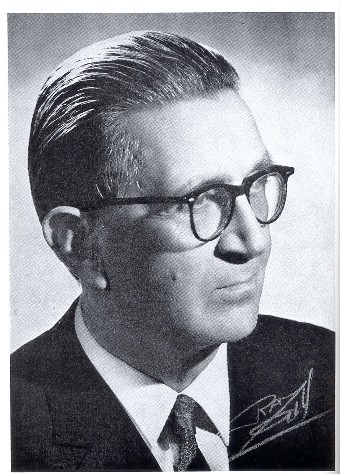
\includegraphics[width=.9\textwidth]{figures/martinet-2.jpg}
  \caption{André Martinet}
  \label{fig:ch.martinet.martinet2}
\end{wrapfigure}
From the presumed vocal character of language, {\Martinet} also derives
the conclusion that linguistic structure, both in the arrangement of
content units (monemes) and the components of their phonic expression
(phonemes), is exclusively successive and linear. Even disregarding
the fact that in signed languages components of both sorts are
frequently simultaneous rather than sequential, this disregards the
fact that spoken languages often display explicitly non-concatenative
morphology, or non-successive combination of meaningful elements. In
\ili{English} pairs such as \emph{sit}/\emph{sat},
\emph{fight}/\emph{fought}, etc. for example, the expressions
of the meanings of the past tense and of the lexical verb are
simultaneous rather than sequential.

The characterization of `language' cited above also makes explicit
{\Martinet}'s rejection of the notion that there are interesting and
important \isi{universals} across languages.  This shows up most directly in
his repeated rejection of {\Jakobson}'s proposals and search for
\isi{universals} as the basis of \isi{regularities} in the structure and
development of individual languages.

The two points with which {\Martinet} is most closely associated,
however, are (1) the conception of language as an instrument of
communication, such that the structure of any particular language is
to be derived from the individual and local ways in which its
components function to serve this purpose within a particular 
community of speakers; and (2) the notion that
human languages display a double \isi{articulation}: on the one hand,
meaningful elements of content (monemes) combine to provide
expressions for an unbounded range of complex meanings, and on the
other, separately meaningless phonemes combine to provide the phonic
forms that signal the identity of particular monemes. The consequences
of the functional commitment will be addressed below; I first take up
the notion of the double \isi{articulation} of language.

\citet{martinet49:double.articulation} was probably the first to
cite this as a criterial feature of human language, although it came to wider
attention in the form of one of {\Hockett}'s ``design features'' of human
language
\citep{hockett58:textbook,hockett:design_features,hockett.ascher64:human.revolution}
as opposed to animal communication systems. A concise statement of
{\Hockett}'s understanding of the principle is the following:

\begin{quotation}
  The utterances of a language consist wholly of arrangements of
  elementary signaling units called \emph{phonemes} (or
  \emph{phonological components} to be exact), which in themselves
  have no meanings but simply serve to keep meaningful utterances
  apart. Thus, an utterance has both a structure in terms of these
  meaningless but differentiating elements, and also a structure in
  terms of the minimum meaningful elements. This design feature is
  \emph{duality of patterning}.\\
  \citep[139]{hockett.ascher64:human.revolution}
\end{quotation}

The basic distinction between two sorts of structure, one composed of
meaningful elements and the other of meaningless elements that serve
to signal these, probably goes back in both cases to {\Hjelmslev}'s
distinction between the content and expression planes, composed of
\emph{pleremes} and \emph{cenemes} respectively. Although neither
{\Martinet} nor {\Hockett} is explicit about this source, {\Martinet} was
certainly quite familiar with {\Hjelmslev}'s theories, and {\Hockett}
actually refers in some places \citep[e.g.][574]{hockett58:textbook}
to the meaningless elements of phonemic structure as \emph{cenemes}.

Neither {\Martinet} nor {\Hockett} explicitly refers to the other's
formulation, but in later work {\Martinet} does provide an almost willful
misinterpretation of what is fairly clearly intended to be {\Hockett}'s
view:

\begin{quotation}
  Some linguists have been using the phrase ``duality of patterning''
  for what we call double \isi{articulation}. The point of view is not the
  same and the implications probably differ. Duality of patterning
  just points to the existence of two different procedures, one for
  isolating phonemes and another one for isolating significant
  segments in the utterance.\\
  \citep[34]{martinet84:double.articulation}
\end{quotation}

Regardless of these matters of intellectual priority, it is
important to see the principle involved as what in substance makes
``phonology'' an essential component of the architecture of human
language. It is tempting to see the presence of phonology as simply an
ornament, an inessential elaboration of the way basic meaningful units
are formed.  This would be a mistake, however: it is phonology, as the
expression of one side of language's double \isi{articulation}, that makes
it possible for speakers of a language to expand its vocabulary at
will and without effective limit.  If every new word had to be
constructed in such a way as to make it holistically distinct from all
others, our capacity to remember, deploy and recognize an inventory of
such signs would be severely limited, to something like a few
hundred. As it is, however, a new word is constructed as simply a new
combination of the inventory of familiar basic sound types, built up
according to the \isi{regularities} of the language's phonology.  This is
what enables us to extend the language's lexicon as new concepts and
conditions require.

The notion of one \isi{articulation} of linguistic structure as based on
recurrent meaningless elements does not by itself, as
\citet{ladd14:duality} makes clear, ensure this productivity. Some
animal communication systems involve expressions composed of
recurrent, meaningless components: zebra finch songs
\citep{lawson.etal18:zebra.finch.song} are built up from a repertoire
of individual syllables, for instance, though the combinations are limited and
different combinations always correspond to the same message. But the
existence of a layer of structure composed of such meaningless
elements allows for the possibility, realized in human languages
although not elsewhere, that the combinatorics of these elements
provides for an open range of possible, distinct expressions, and this
is the role of phonology in linguistic structure.

The task of phonology, then, is to uncover and explore the system of
the ``second \isi{articulation}'' in individual languages, that is, the
inventory and combinatory possibilities of the language's set of
phonemes. A relatively standard approach to this within structuralist
theories would be to collect a corpus of utterances in a phonetic
representation, and then explore the inventory of phonetic segments
found there to see which ones \isi{contrast} with one another (and thus belong
to distinct phonemes) and which do not (and are thus candidates for
allophones of the same \isi{phoneme}). {\Martinet}, however, rejects such an
approach, on the grounds that the \isi{segmentation} present in the presumed
\isi{phonetic representations} is not objectively systematic, but rather
strongly dependent on the background, experience and native language
of the transcriber. This objection is interestingly similar to one
raised by {\Bloomfield}, which will be discussed below in
section~\ref{sec:bloomfield-representations}.

{\Martinet} proposes to identify phonemes through the process he refers
to as \emph{commutation}, echoing {\Hjelmslev}'s terminology. In
analyzing the phonology of a language, the linguist begins with a
collection of convenient sized utterances --- typically single words
--- and compares them to focus on indivisible, minimal sized portions
whose difference results in a change of \isi{meaning}. This does not require
an analysis of meanings, but only recourse to a notion of
\emph{difference} in \isi{meaning}. This analysis is carried out with
respect to a range of contexts, with a set of elements identified for
each that function to differentiate \isi{meaning}, and thereby to contribute
to the functioning of a language as a tool to convey \isi{meaning} among its
speakers.\footnote{It is not clear that {\Martinet} actually arrived at
  his analyses of \ili{Danish} \citep{martinet37:danish}, \ili{French} (lecture 3
  in \citealt{martinet49:functional.phonetics} and elsewhere), or the
  \ili{Franco-Provençal} of Hauteville \citep{martinet56:description} by
  anything like the process of commutation he describes. His analyses
  appear to proceed in the standard way from an inventory of phonetic
  segments, to explore the dimensions of functional \isi{contrast} among
  them.}

For example \citep[63ff.]{martinet65:synchronique}, comparing \ili{French}
\emph{banc, pan, van, faon, dent, temps, zan, sang, gens, champ, gant,
camp, lent, rang, ment} we can identify 15 distinctive units in
initial position before {[ã]}, units which we could designate with the
letters \emph{b, p, v, f} etc. Comparing \emph{bout, pou, vous, fou,
  doux, toux, zou, sou, joue, chou, goût, cou, loup, roue, mou} we can
again identify 15 units, this time before {[u]}, which we are tempted
to designate with the same letters \emph{b, p, v, f} etc.

But what justifies the identification of, e.g., the initial element of
\emph{banc} with that of \emph{bout}? The answer that immediately
suggests itself is their phonetic similarity, but this is not what
establishes them as the same \isi{phoneme} for {\Martinet}. What matters for
him is that the \emph{b} of \emph{banc} is differentiated from the
\emph{p} of \emph{pan}, the \emph{v} of \emph{van}, and the \emph{d}
of \emph{dent} by the same relevant properties (voiced as opposed to
voiceless, stop as opposed to fricative, labial as opposed to apical)
as the \emph{b} of \emph{bout} is to the \emph{p} of \emph{pou}, the
\emph{v} of \emph{vous} and the \emph{d} of \emph{dent}. The identity
of a \isi{phoneme}, that is, resides not in its positive phonetic
properties, but rather in the set of relevant features that give it
its communicative function by differentiating it from others in the
same environment.

A \isi{phoneme}, then, is to be equated with a set of distinctions, and not
directly with a phonetic value. This is illustrated, for instance, in
the analysis of \ili{Danish}. In that language, vowels are systematically
lower in certain /r/ contexts. As a result \citep[60]{martinet64:elements}
``the \isi{phoneme} /æ/ is manifested as {[ɛ]} in \emph{net} `pretty' but as
{[a]} in \emph{ret} `correct, right'; the sound {[a]} which is the
manifestation of the \isi{phoneme} /æ/ in \emph{ret} is the manifestation of
another \isi{phoneme} /ɑ/ in \emph{nat} `night'.'' The point is that \ili{Danish} distinguishes four
degrees of vowel height in certain /r/ contexts and elsewhere, but the
phonetic value of the vowel is lower in these /r/ contexts than
elsewhere. As a result, the lowest vowel of the series /i, e, æ, ɑ/ is
phonetically the same in other environments as the next-to-lowest
vowel in those /r/ contexts. The same phonetic value can thus
correspond to more than one phonemic unit, and conversely, a single
\isi{phoneme} can be manifested in more than one way phonetically. What
characterizes a given \isi{phoneme} is therefore not its phonetic identity
\emph{per se}, but rather the contrastive value it exhibits with
respect to \isi{oppositions} distinguishing it form others in the same
position.

The phonematic system of a language consists not simply of an
inventory of the phonemes established through an analysis of
contrastive function, but more importantly, echoing {\Martinet}'s Prague
School background, of the set of dimensions on which \isi{contrast} occurs,
the set of \isi{oppositions}. {\Martinet}'s classification of these also echoes
e.g. that of \citet{trubetzkoy39:grundzuge}, discussed above in
section~\ref{sec:structure-of-systems}. In some cases, exactly two
phonemes \isi{contrast} on a given dimension at a time, as in the case of
voiced \emph{vs.}  voiceless phonemes in \ili{French} (/b/ \emph{vs.}  /p/,
etc.), a \emph{bilateral} opposition.  Other \isi{oppositions}, however, are
\emph{multilateral}, in that they involve more than two values: for
instance the dimension of \isi{place of articulation}, opposing labial,
apical, palatal and velar phonemes that are otherwise similar in their
relation to others. When the same binary opposition distinguishes
corresponding pairs of phonemes in two parallel series, as with /b/
\emph{vs.} /p/, /v/ \emph{vs.} /f/, /d/ \emph{vs.}  /t/, etc., each of
which exists, in {\Martinet}'s terms, by virtue of its \isi{contrast} with the
other, the relation between the two opposing series is called a
\emph{correlation}.

{\Martinet}'s embrace of irreducible multilateral \isi{oppositions} aligns him
with {\Trubetzkoy}'s practice, and sets him in opposition to {\Jakobson}'s
efforts to reduce all multilateral \isi{oppositions} to complexes of
strictly binary ones. This became a significant point of contention
between them, and {\Martinet} wrote many times of his rejection of the
``apriorism'' of {\Jakobson}'s attempt to enforce strict binarity on the
structure of phonological systems.

Given the similarity between {\Martinet}'s account of phonological
structure and that of {\Trubetzkoy}, it comes as no surprise that
{\Martinet} also includes provision for a quite similar notion of
archiphonemes, units that represent the \isi{neutralization} of a phonemic
\isi{contrast} in certain positions. The standard example is the
\isi{neutralization} of obstruent \isi{voicing} distinctions in syllable-final
position in \ili{German} and \ili{Russian}. While the phonemes /d/ and /t/ are
distinct in \ili{German} in the position before a vowel, in final position
there is no \isi{contrast}, and the words \emph{Rad} `wheel' and \emph{Rat}
`advice' are pronounced identically as {[rat]}. In such a case the
final segment is neither /d/ nor /t/, since the choice of either would
imply a \isi{contrast} with the other.  Rather, it is an \isi{archiphoneme} which
we can write as /T/, consisting of the relevant features \{apical,
stop\} with no value for the feature voiced \emph{vs.} voiceless.

In such a case, we say that the feature voiced is \emph{neutralized}
in (syllable-)final position in \ili{German}, with obstruents represented by
an \isi{archiphoneme} lacking a value for voiced. It will be recalled that
{\Trubetzkoy} (section~\ref{sec:neutralization}) maintained that only
bilateral \isi{oppositions} could be neutralized in an \isi{archiphoneme},
offering an incorrect argument to that effect. {\Martinet} provides a
similar argument, but uses it instead to show that not all instances of
\isi{defective distribution} should be represented by archiphonemes. Thus,
in \ili{English} /l/ appears following initial /p, b/ and also /k, g/
(\emph{plan, bland, clan, gland}) but not after initial /t, d/. To
represent, say, the fact that there cannot be a word \emph{*tlan,
  *dland} by writing the initial of \emph{plan, bland} as
archiphonemic /Plæn, Blænd/ and defining /P, B/ as the \isi{neutralization}
of /p/ and /t/, /b/ and /d/ respectively would be a mistake, since it
would imply that this segment has no value for \isi{place of articulation},
while it does indeed \isi{contrast} with the /k, g/ of \emph{clan, gland}.

This argument does not show, as claimed by {\Trubetzkoy}, that
multilateral \isi{oppositions} such as articulatory place cannot be
neutralized and represented by an \isi{archiphoneme}. Rather, it shows that
such a \isi{neutralization} must affect all of the members of the
opposition, and not just some of them. \ili{Spanish}, for instance, has
three phonemically distinct nasals at the beginning of a \isi{syllable}, as
shown by the \isi{contrast} among \emph{cama} `bed', \emph{cana} `gray
hair', and \emph{caña}`cane'.  Before a labial consonant, however,
only {[m]} can appear, as in \emph{campo} `field'; before an alveolar
consonant, only {[n]}, as in \emph{insipido} `tasteless', and before a
palatal, only {[ɲ]}, as in \emph{ancho} `broad'. Since all of the
terms of the place opposition are neutralized before a consonant, we
can represent these phonemically as /ˈkaNpo/, /iNˈsipido/ and /ˈaNčo/
respectively.

\ili{English} also has three phonemic nasals: /m, n, ŋ/ as in \emph{ram, ran,
  rang}. The contrasts among these are neutralized, as in \ili{Spanish},
before a final stop consonant, and it obviously suggests itself to
represent e.g. \emph{ramp, rant, rank} as /ræNp/, /ræNt/,
/ræNk/. Notice, however, that on a purely representational view such
as {\Martinet}'s, there is nothing to prevent the somewhat
counter-intuitive interpretation of the nasals here as maintaining
their phonemic value, while treating the final \isi{stops} as represented by
an \isi{archiphoneme} /T/ `voiceless stop', with place information depending
on the preceding nasal: thus, /ræmT/, /rænT/, /ræŋT/.

This analysis can be excluded in a rule-based account of \ili{Spanish},
because in e.g. \emph{un beso} `a kiss' {[umbeso]}, \emph{un tipo} `a
type' {[untipo]}, \emph{un chubasco} `a heavy shower' {[uɲčubasko]},
\emph{un gato} `a cat' {[uŋgato]} a rule assimilating \isi{nasal consonants}
to following obstruents, including velars with no corresponding
phonemic nasal, is clearly motivated. In {contrast} with the \ili{English}
case, the phonemic identity of the second word in the sequence,
together with the absence of phonemic /ŋ/, precludes the analysis
assimilating its initial to the preceding nasal. Since the rule thus
established also accommodates the intra-morphemic cases, there is no
reason to treat these differently. It is more difficult to apply this
argument in \ili{English}, however, since nasal \isi{assimilation} has a somewhat
different status in this language.

A universalist theory of phonology might argue from the fact of the
regressive, anticipatory \isi{assimilation} of nasals to following
\isi{consonants} in \isi{place of articulation}, combined with the general absence
of \isi{assimilation} in the opposite direction (from the nasal to the
following consonant) that the asymmetry is due to something in the
architecture of phonological systems. On that basis, the
counter-intuitive analysis of the \ili{English} facts suggested above could
be excluded. On a radically particularist view such as {\Martinet}'s
however, nothing about \ili{Spanish} or any other language could be seen as
relevant to the analysis of \ili{English}.
  
{\Martinet} recognizes that \isi{neutralization} in an \isi{archiphoneme} often
provides a description of an \isi{alternation}. In \ili{French}, the vowels /e/
and /ɛ/ are in \isi{contrast} in final position, as in \emph{gré} {[gre]}
`wish, desire' \emph{vs.} \emph{grès} {[grɛ]} `sandstone'. Medially,
however, the opposition is neutralized, with only {[e]} appearing in
an open \isi{syllable} (e.g. \emph{rep\underline{é}ter}
{[rəp\underline{e}te]} `to repeat' vs. \emph{ (il) rep\underline{è}te}
{[rəp\underline{ɛ}t]} `(he) repeats' with {[ɛ]} in a closed \isi{syllable}. 
In such a case, an \isi{alternation}
(e/ɛ) appears and is represented by an \isi{archiphoneme}.  {\Martinet} is
quite explicit, however, that this is only possible for a very
restricted set of alternations: instances in which the alternating
segments differ only as the terms of a completely neutralized
opposition, and where the conditioning of the choice is entirely due
to the phonological environment.

He is quite clear that other alternations, such as that of ø/u in
\emph{ils p\underline{eu}vent}/\emph{nous p\underline{ou}vons}
`they/we can' or ɛ̃/in in
\emph{cop\underline{ain}}/\emph{cop\underline{ine}} `friend/girl
friend' are not to be treated in parallel fashion. In these cases the
choice of one value \emph{vs.} the other is based on morphological,
and not phonological factors, and thus has nothing to do with
phonology. In several places, indeed, {\Martinet} criticizes {\Trubetzkoy}
for having included the notion of `morpho(pho)nology' in his conception
of phonology. The absolute exclusion of anything but the simplest of
automatic alternations from the domain of phonology establishes rather
clearly that this is a theory of \isi{representations} and not of rules.

{\Martinet}'s writing on phonological topics devotes considerable
attention to the description and analysis of prosodic properties ---
linguistic uses of \isi{pitch}, \isi{accent}, etc., properties whose scope is not
in general that of a single phonemic segment, but rather a \isi{syllable},
word, or other stretch of an utterance.  A full account of his views
would require extensive discussion of these matters, but for present
purposes the above description of his central positions on phonematics
will suffice.


\section{Functional factors in phonological change}
\label{sec:economie}

Although in some sense phonology as a coherent object of study has its
origins in Saussure's insistence that a science of language has to
focus on achieving an understanding of the character of synchronic
systems, that does not at all mean that linguistic diachrony
disappeared from view. Recall that Saussure himself
(chapter~\ref{ch.saussure_life}) was widely known for his
\textsl{Mémoire}, a work that revolutionized historical \ili{Indo-European}
studies, and the few other works directly from his pen mostly
concerned historical topics (especially Baltic accentuation). Baudouin
de Courtenay (chapter~\ref{ch.kazan}) was also known as a historical
linguist and as noted there developed a view of \isi{historical change} in
the character of alternations on the basis of his understanding of
their synchronic \isi{typology}. A major obsession of Trubezkoy's
(chapter~\ref{ch.prague}) throughout his life was the project of a
definitive \textsl{Prehistory of Slavic}, and one of the goals of the
\textsl{Grundzüge} was an understanding of \isi{universals} of sound
structure that would underpin an explanatory theory of diachronic
change. As was shown in chapter~\ref{ch.jakobson}, {\Jakobson} continued this attention to
the interplay between synchronic principles and \isi{historical change}.

Among the pioneers of phonological study in America that we will
consider in later chapters, {\Sapir} (chapter~\ref{ch.sapir}) wrote much
on historical topics and insisted that his students working on the
indigenous languages of the Americas attend to the implications of
their results for comparative studies.  {\Bloomfield}
(chapter~\ref{ch.bloomfield}) was also focused on historical
relationships, especially among the \ili{Algonquian} languages, and one of
his more important results was the demonstration in
\citealt{bloomfield25:algonquian} that the principles of diachronic
change were as applicable to unwritten languages as they were to the
familiar languages of \ili{Indo-European} scholarship.

\begin{wrapfigure}[13]{l}{.3\textwidth}
  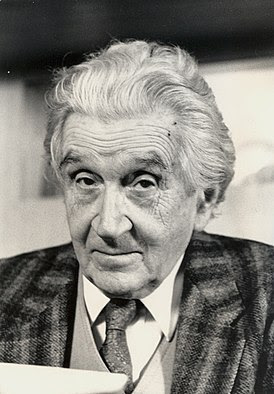
\includegraphics[width=.9\textwidth]{figures/martinet-3.jpg}
  \caption{André Martinet}
  \label{fig:ch.martinet.martinet3}
\end{wrapfigure}
While I have paid little attention to historical work
in this book, a proper appreciation of the development of phonology
must include consideration of the implications phonologists have
seen of their understanding of synchronic \isi{regularities} for processes
of historical
change. \citet{martinet52:function.structure,martinet55:economie} is
particularly notable in this regard for providing a well worked out account of
diachronic development as a consequence of the character of individual
phonological systems. As in the case of his views on synchronic
phonology, however, the emergence of his views on diachrony should be
seen in part against the background of {\Jakobson}'s work.

Throughout his career, {\Jakobson} was concerned with the interplay of
synchronic and diachronic principles, perhaps most extensively
developed in \citealt{jakobson29:remarks} (recently translated into
{English} with notes as \citealt{jakobson18:remarks}).
\citet{jakobson49:historical} provides a convenient summary of what he
saw as the most important relations between these domains.

{\Jakobson} saw phonological systems as grounded in a system of
\isi{universals}, with a limited set of universally available binary
\isi{oppositions} defined in a way independent of any particular language,
the system of \isi{distinctive features}, playing a central role. The
\isi{distinctive features} were not taken to be completely independent of
one another, and a number of implicational relations among them were
assumed to govern individual phonologies. For example, he argued that
since contrasts of \isi{pitch} and \isi{palatalization} were described in terms of 
a single opposition of "Tonality", they could not in principle be maintained independently.
Another claim was that languages could not sustain an opposition of \isi{free vowel} quantity and
free intensity \isi{accent} together. However, an opposition of one
\isi{pitch} contour to another (e.g. falling vs. rising \isi{tone}s) requires a
language to maintain a \isi{contrast} between long vs. short vowels.

Linguistic changes then, were at least in many cases to be seen as
teleological, taking a language from a state in which one or another
implicational relation among \isi{oppositions} was compromised to one where
it was satisfied. Thus, if some set of circumstances resulted in
previously automatic \isi{stress} becoming unpredictable and free, the
language would need to lose an accompanying \isi{vowel length}
distinction. On the basis of principles of this sort, he provided an
account of a number of superficially unrelated changes in the early
history of the Slavic languages.

{\Martinet} rejected all of the underpinnings of {\Jakobson}'s view:
languages were taken to be the completely idiosyncratic communication
systems in use in individual speech communities, with no necessary
comparability and certainly no basis in a collection of \isi{oppositions}
defined independently. Nonetheless, he did maintain a number of
characteristics of phonological systems toward which languages might
be seen to strive. Rather than being grounded in a presumed universal
framework, though, these were argued to follow from the basic function
of language as a means of communication.

{\Martinet}'s discussion of the mechanisms of phonological change and
their motivations involves and invokes a number of concepts familiar
from the work of others. This includes the notion of ``least effort''
for example, and the constant tension between the need of speakers to
minimize the effort involved in speaking and that of hearers to
recover the distinctions keeping meaningful units separate. He also
recognizes the importance of the mutual, syntagmatic influence of
adjacent elements in the speech chain which tend to accommodate to one
another. Principles of this nature were, of course, the basis of
phonetic explanations in Neogrammarian theories, and they maintain
considerable importance in any account of phonological diachrony.

An individually distinctive aspect of {\Martinet}'s theorizing about
phonological change, however, was his emphasis on the phonemic
elements of a language as forming a dynamic system grounded in
communicatively functional contrasts, rather than a simple inventory
of distinctive elements. Phonemes differ from one another in terms of
their characteristic features, and these features organize the
phonemes into a coherent pattern of \isi{oppositions}, series, \isi{correlations},
bundles of \isi{correlations}, etc.  Since it is \isi{phoneme} \emph{systems} and
not just their individual members that constitute the phonology of a
language, it follows that the properties of such a system play a role
in change. This results in a tendency to maximize the symmetry of the
system by extending \isi{correlations}, filling structural gaps, etc.

Importantly also, a \isi{phoneme} cannot be identified with a single, constant
phonetic value, since it must be implemented physically and 
physical events are never totally identical, and therefore each \isi{phoneme} is
associated with a range of possible implementations. Since the
communicative function of a \isi{phoneme} is to be distinguishable from
others, the ranges of similar phonemes must maintain enough separation
from one another to support this. As a result, {\Martinet} proposes that
the phonemes of a language will tend to have ranges of implementation
that are maximally separated, a notion that would appear in much later
theorizing about phonological systems as ``Dispersion Theory'' or the
like (\citealt{liljencrants.lindblom72:dispersion} and many other
references).

The tendencies to maximize system symmetry and to distribute phonemes
evenly in phonetic space must be seen against the background of
asymmetries in that space. Thus, if a language has four degrees of
height in the front vowel system, we expect a tendency to have four
heights also in the back vowels, but in fact the articulators provide
less space for height \isi{variation} in the back of the mouth than in the
front, and thus there is pressure for back vowels to be fronted. This
is most likely for higher vowels, since again there is more
articulatory space for high vowels than for low. We thus find changes
such as the fronting of /u/ to {[ü]} in \ili{French}, \ili{Icelandic}, and other
languages.

At any given time, the phonetic values for a given \isi{phoneme} will fall
within a particular range, and this range may be subject to some
\isi{variation}. Suppose we have two phonemes /A/ and /B/ with ranges that
are close but which do not overlap. Now suppose that the
implementations of /A/ shift somewhat over time, so as come closer to
or even overlap with the range of /B/. There are two possible
outcomes: one is for the \isi{contrast} between /A/ and /B/ to be lost, and
for the two to collapse as one. The other is for the range of /B/ to
shift enough to restore the required separation that supports their
functional distinctness.

Which of these developments will occur in a given case is driven in
large part, according to {\Martinet}, by the ``functional yield'' (or
``functional load'') of the opposition between /A/ and /B/, that is,
by the importance of this particular distinction in separating
distinct monemes of the language. He admits that this is a very
difficult \isi{concept} to make precise: neither the type frequency of
monemes distinguished by /A/ vs. /B/ nor the \isi{token} frequency of these
monemes in texts is really satisfactory, and the question of how the
opposition between them is integrated into the overall pattern of
series, \isi{correlations}, etc. of the phonemic system also plays a
role. Nonetheless, it is intuitively appealing that \isi{oppositions} are
less likely to be neutralized in this way to the extent they are
well integrated into the language's phonemic system and
important to the functional separation of meaningful elements.

If the functional yield of the \isi{contrast} between /A/ and /B/ is high
enough that it should be maintained, on the other hand, the
encroachment of /A/'s range into that of /B/ will naturally result in
/B/ shifting its range, too, so as to restore the required degree of
separation. And perhaps this will result in /B/ approaching the range
of another \isi{phoneme} /C/, thus motivating a further shift in the
implementations of this element, and so on. Such a collection of
changes, initiated by a shift in the range of /A/ toward that of /B/
and so on, constitutes a ``\isi{push chain}'', an important notion deriving
from {\Martinet}'s work.

Alternatively, suppose that the range of implementation of /A/ shifts
so as to be further from that of /B/. In that case, in order to
maintain a maximal dispersion of phonemic elements in phonetic space,
/B/ might shift toward /A/, taking up some of the space thus left
vacant; and a nearby /C/ might then shift toward /B/ for similar
reasons, etc. In this case, where the set of changes is initiated by
one \isi{phoneme}'s moving away from another, we have a ``\isi{pull chain}''.

{\Martinet} (and others following in his footsteps) analyze a large
number of developments of the sort just described, and it is clear
that such correlated changes are not at all rare. In individual
cases, where the precise time course of the various components of the
overall change is hard or impossible to establish, it is typically
difficult to distinguish in a specific instance whether we have to do
with a \isi{push chain} (initiated by a change in the first element /A/ of a
shift /A/→/B/→/C/ etc.) or a \isi{pull chain} initiated by the last element
/C/, although conceptually the distinction is clear.

{\Martinet}'s notions of the factors involved in phonological change were
passed on at Columbia via his student \name{Uriel}{Weinreich} to {\Weinreich}'s
student, \name{William}{Labov}, in whose work they were considerably
developed. \posscitet{labov66:stratification} classic study of the
dimensions of \isi{variation} in the \ili{English} of New York City initiated a
broad and very productive research program that has in many instances
fleshed out {\Martinet}'s ideas about the role of \isi{variation} in
change. {\Martinet}'s influence is very strong in
\posscitet{labov94:ling.change.1,labov01:ling.change.2,labov10:ling.change.3}
comprehensive account of the factors shaping diachronic change in
phonological systems.

{\Martinet}'s continuing influence on thinking about the ``second
\isi{articulation}'' of linguistic structure is largely confined to
historical work of this sort. The importance of
\citealt{martinet55:economie} in this regard is quite generally
recognized, and his role in drawing attention to the significance of
\isi{variation} in phonological structure can be credited with shaping
contemporary views of the sociolinguistics of phonological form.


%%% Local Variables: 
%%% mode: latex
%%% TeX-master: "/Users/sra/Dropbox/Docs/Books/P20C_2/LSP/main.tex"
%%% End: 
